\documentclass[letterpaper,11pt]{article}
\oddsidemargin -1.0cm \textwidth 17.5cm

\usepackage[utf8]{inputenc}
\usepackage[activeacute,spanish, es-lcroman]{babel}
\decimalpoint
\usepackage{amsfonts,setspace}
\usepackage{amsmath}
\usepackage{amssymb, amsmath, amsthm}
\usepackage{comment}
\usepackage{float}
\usepackage{amssymb}
\usepackage{dsfont}
\usepackage{anysize}
\usepackage{multicol}
\usepackage{enumerate}
\usepackage{graphicx}
\usepackage[left=1.5cm,top=2cm,right=1.5cm, bottom=1.7cm]{geometry}
\setlength\headheight{1.5em} 
\usepackage{fancyhdr}
\usepackage{multicol}
\usepackage{hyperref}
\usepackage{wrapfig}
\usepackage{subcaption}
\usepackage{siunitx}
\usepackage{cancel}
\usepackage{mdwlist}
\usepackage{svg}
\pagestyle{fancy}
\fancyhf{}
\renewcommand{\labelenumi}{\normalsize\bfseries P\arabic{enumi}.}
\renewcommand{\labelenumii}{\normalsize\bfseries (\alph{enumii})}
\renewcommand{\labelenumiii}{\normalsize\bfseries \roman{enumiii})}


\begin{document}

\fancyhead[L]{\itshape{Facultad de Ciencias F\'isicas y Matem\'aticas}}
\fancyhead[R]{\itshape{Universidad de Chile}}
\rfoot[]{pág. \thepage}

\begin{minipage}{11.5cm}
    \begin{flushleft}
        \hspace*{-0.6cm}\textbf{FI1000 Introducción a la Física Clásica}\\
        \hspace*{-0.6cm}\textbf{Tutor:} Alejandro Cartes
    \end{flushleft}
\end{minipage}

\begin{picture}(2,3)
    \put(366, -10){
\includegraphics[scale=0.9]{2020-1/Imágenes/logo/dfi-fcfm.pdf}}
\end{picture}

\begin{center}
	\LARGE\textbf{Tutoría Examen}
\end{center}

\vspace{-1cm}
\begin{enumerate}\setlength{\itemsep}{0.4cm}

\item[]

\item \textbf{[Hidrostática + Dinámica]} Se tiene un objeto de altura $h$ y área transversal $A$ compuesto por un material de densidad homogénea $\rho$. El cubo está sujeto a un resorte de constante elástica $k$ y largo natural $\ell_0$. Todo el sistema está dentro de un recipiente lleno con un líquido con densidad $\rho_f$ hasta una altura $H$, como se muestra en la figura.
    \begin{enumerate}
        \item Determine la posición de equilibrio del objeto con respecto al fondo del recipiente
        \item Determine que densidad debe tener el objeto para que, en equilibrio, flote semi-sumergido justo hasta la mitad. Comente los casos:
        \begin{itemize}
            \item $\ell_0 > H -\frac{h}{2}$
            \item $\ell_0 = H -\frac{h}{2}$
        \end{itemize}

    \end{enumerate}
    \begin{figure}[H]
        \centering
        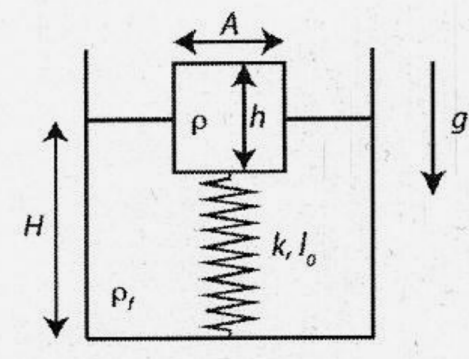
\includegraphics[height=0.3\textwidth]{2023-1/img/aux_16/Aux 16 - P4.PNG}
    \end{figure}

\item 
\begin{multicols}{2}
    \textbf{[Dinámica + Cinemática]} Un bloque de masa $m$ está apoyado sobre la superficie de una cuña, que forma un ángulo $\alpha$ con la horizontal. La superficie de contacto entre ambas superficies está caracterizada por coeficientes de roce estático $\mu_e$ y cinético $\mu_c$, que son suficientemente grandes de manera que el bloque no desliza si la cuña está inmóvil. Mediante una cuerda, la cuña es forzada a moverse hacia la derecha con una aceleración constante $a_0$, tal como se muestra en la figura. 

    \columnbreak

    \begin{figure}[H]
        \centering
        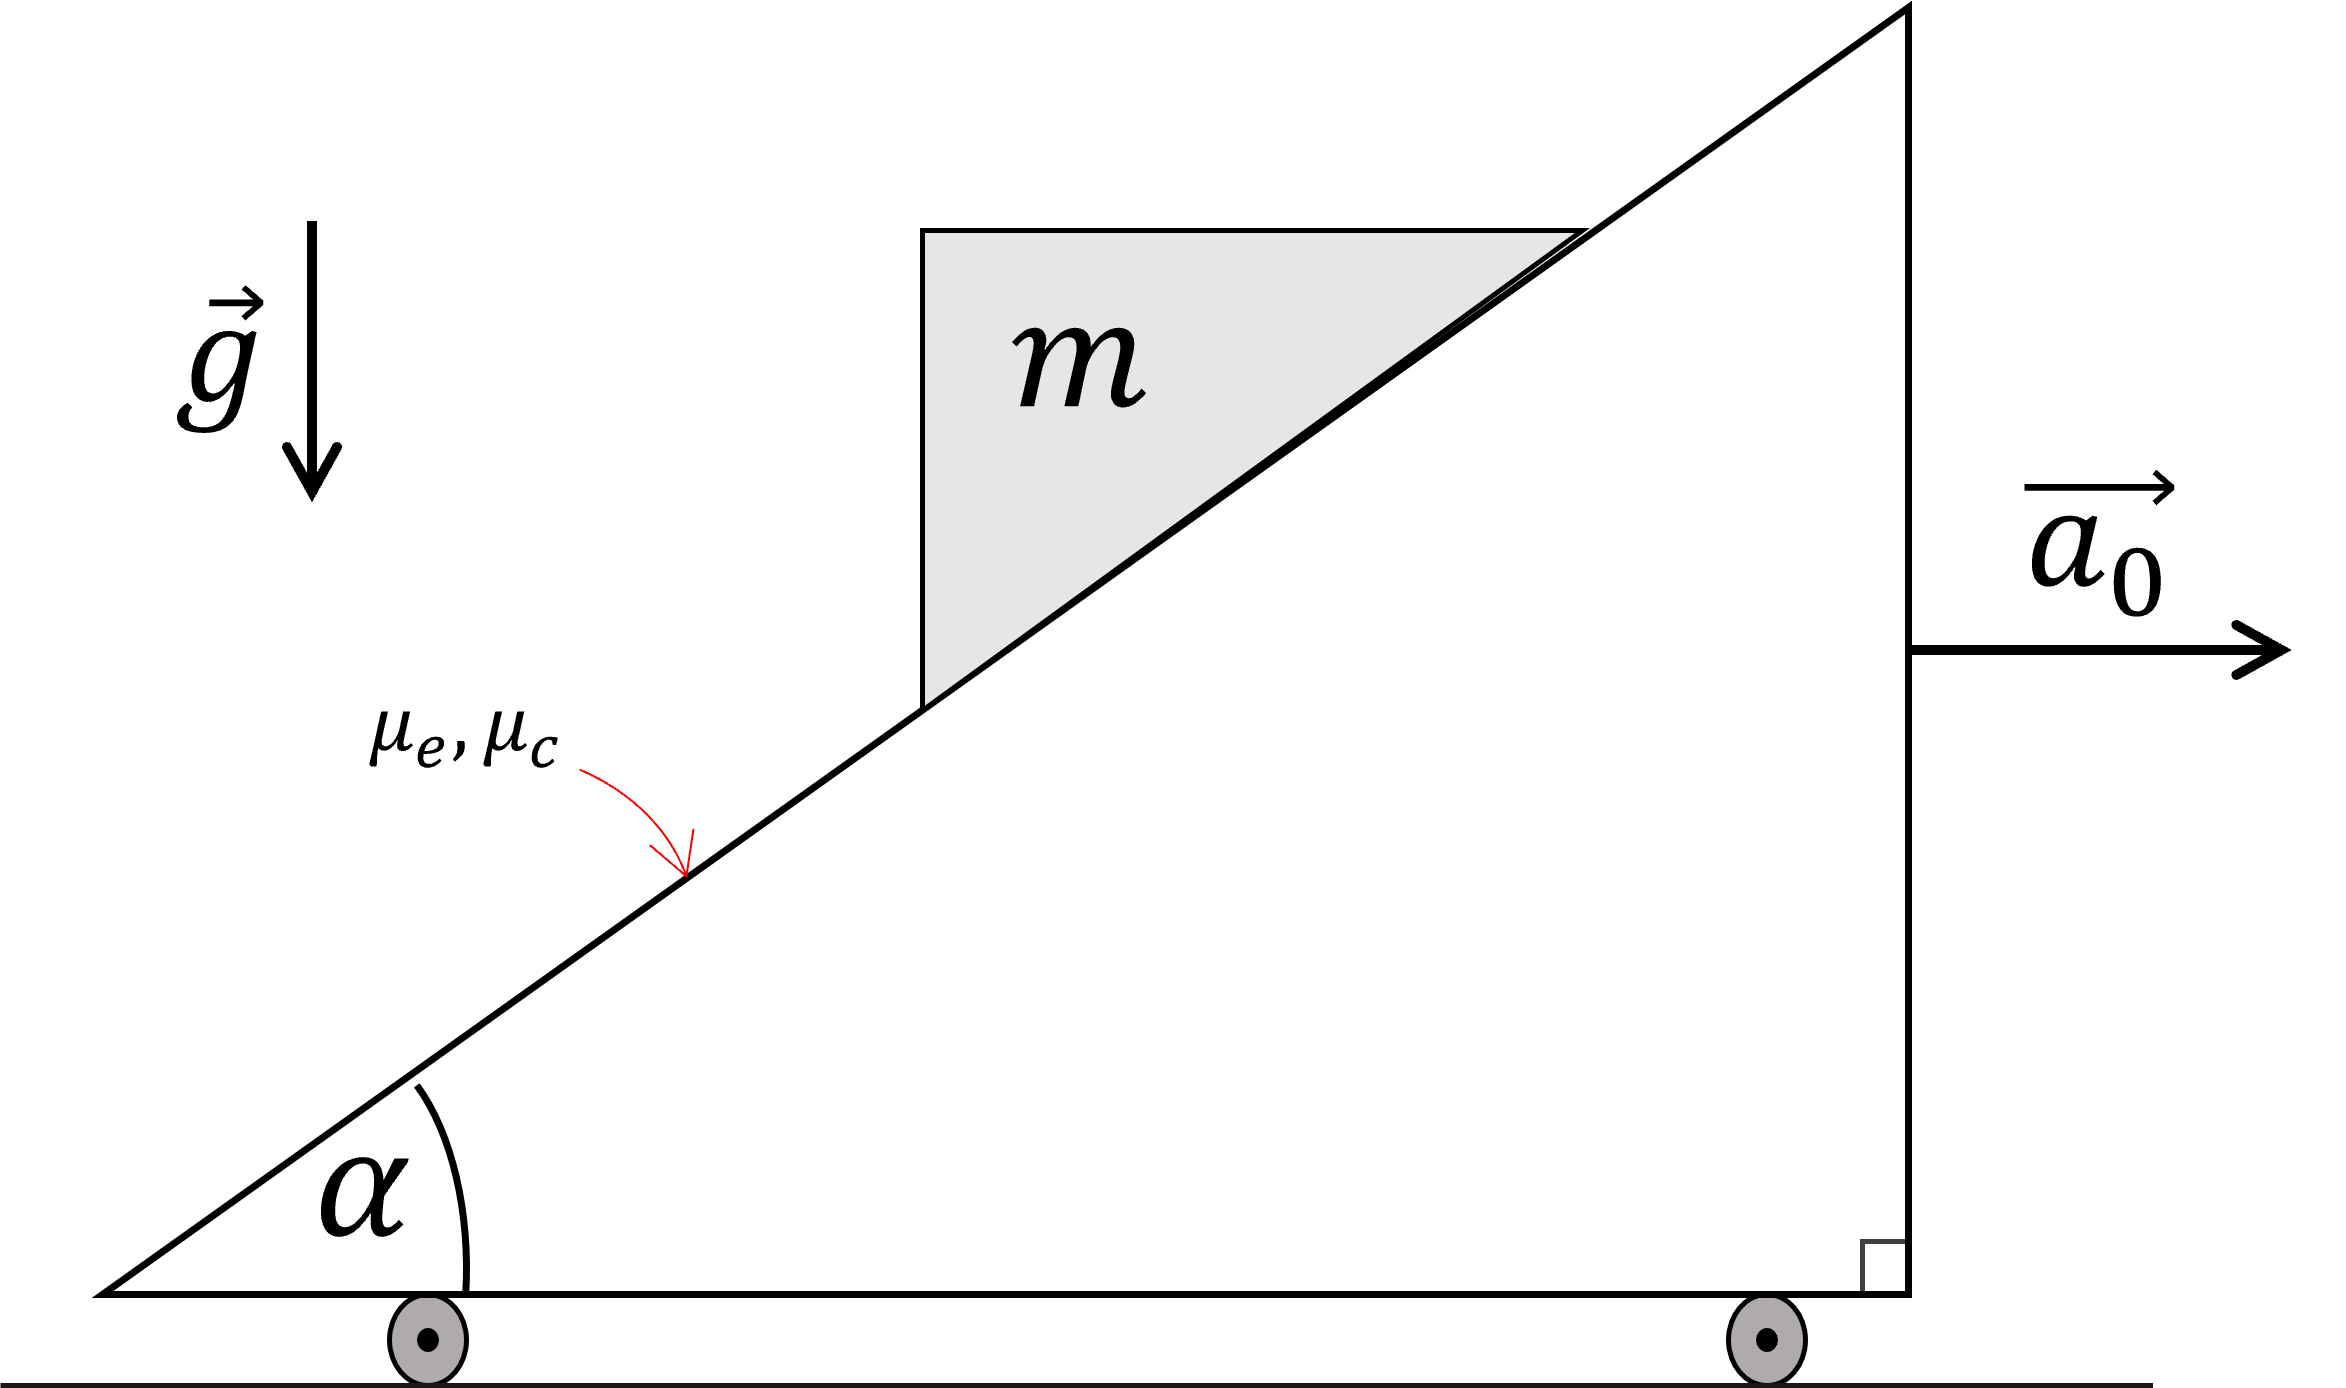
\includegraphics[width=0.8\linewidth]{2022-1/img/cepc/masa cunia.png}
    \end{figure}
\end{multicols}
    \begin{enumerate}
        \item Determine el valor mínimo de $a_0$ de manera que el bloque empieza a deslizar sobre la cuña.
        
        \item Si se cumple la condición encontrada en la parte anterior, calcule la componente vertical de la aceleración del bloque
    \end{enumerate}

% \item Considere un plano horizontal donde reposa un a masa $m$ que se impulsa desde el reposo por una fuerza constante $\vec{F}=F\hat{x}$, la cual actúa por un tiempo $T$. Luego de que la masa alcanza su rapidez máxima, esta comienza a subir por un plano inclinado con ángulo $\theta$, con respecto a la horizontal. A una altura $h$ del plano inclinado se encuentra un resorte ideal en su largo de equilibrio $L_0$, con constante elástica $k_1$, como se muestra en la figura. Determine:

% \begin{enumerate}
%     \item La rapidez de la masa al comenzar a subir por el plano inclinado

%     \item La compresión máxima del resorte en altura debido a la acción de la masa
% \end{enumerate}

\item \textbf{[Momentum + Energía]} Un dispositivo explosivo de masa total $M$ se introduce en un aparato para medir la energía de la explosión. El aparato tiene dos resortes de largo natural $L_0$ y con constantes elásticas $k_1$ y $k_2$. Al activar el explosivo, este se divide en dos como se muestra en la figura.

El fragmento de menor masa $m$ viaja hacia la izquierda y comprime al resorte 1 una cantidad $L_1$. Determine la deformación del segundo resorte por efecto del fragmento de mayor tamaño y la energía total liberada por la explosión

\begin{figure}[H]
    \centering
    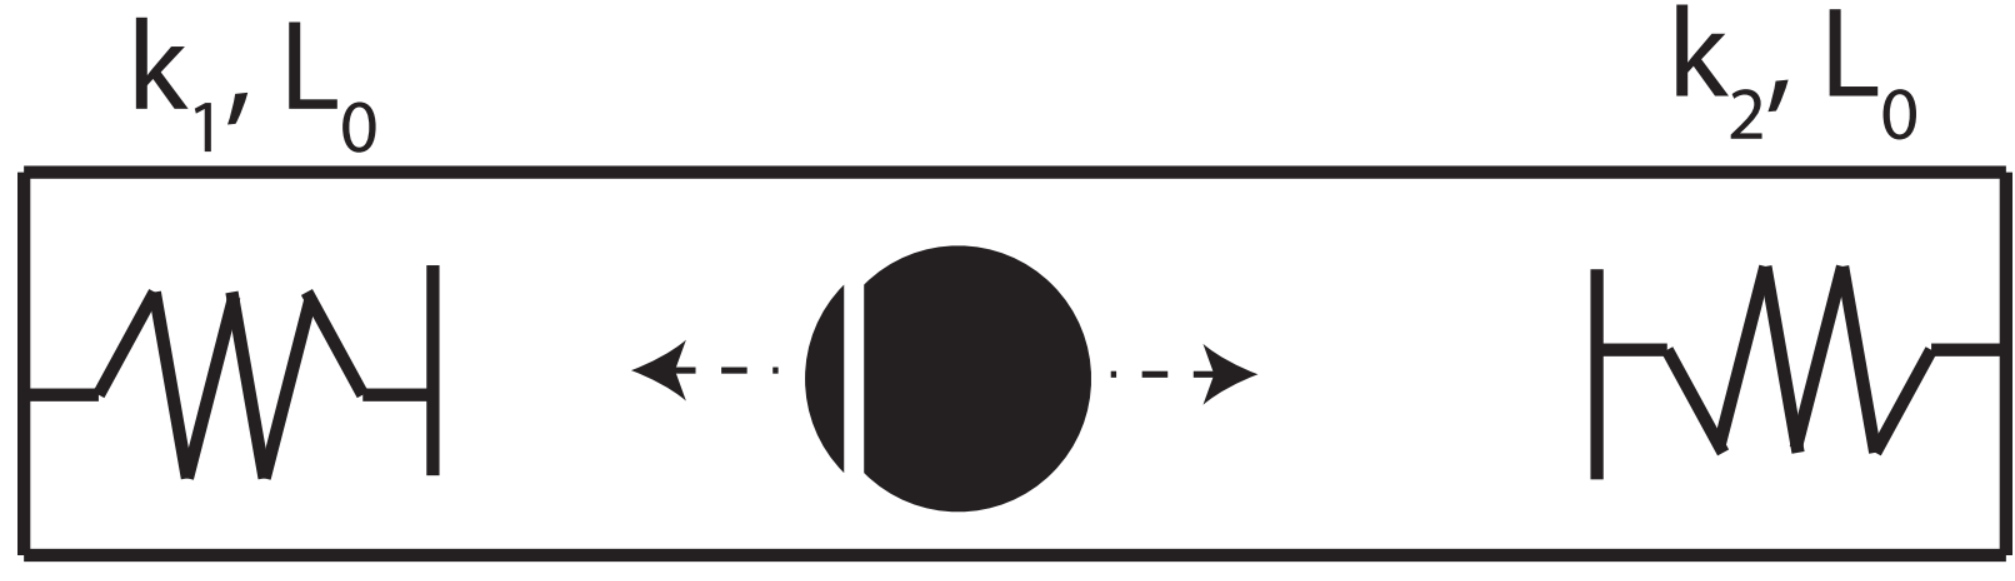
\includegraphics[width=0.5\linewidth]{tutorías/2024/img/dispositivo.png}
\end{figure}

\item \textbf{[Estática]} Un vaso de forma cilíndrica de radio $r$ y altura $h$ se posa sobre un plano inclinado. Para que no resbale se coloca un tope fijo en el plano. Suponga que los puntos de contacto del vaso con la superficie son aquellos ennegrecidos en la figura.

\begin{minipage}{0.6\linewidth}
    Si el ángulo de inclinación del plano es $\beta$, determine:
    \begin{enumerate}
        \item La posición del centro de masa con respecto al punto de contacto $O$
    
        \item La fuerza normal en cada punto de contacto
    
        \item El ángulo de inclinación máximo del plano de modo que el vaso no vuelque
    \end{enumerate}
\end{minipage}
\hfill
\begin{minipage}{0.3\linewidth}
    \begin{figure}[H]
        \centering
        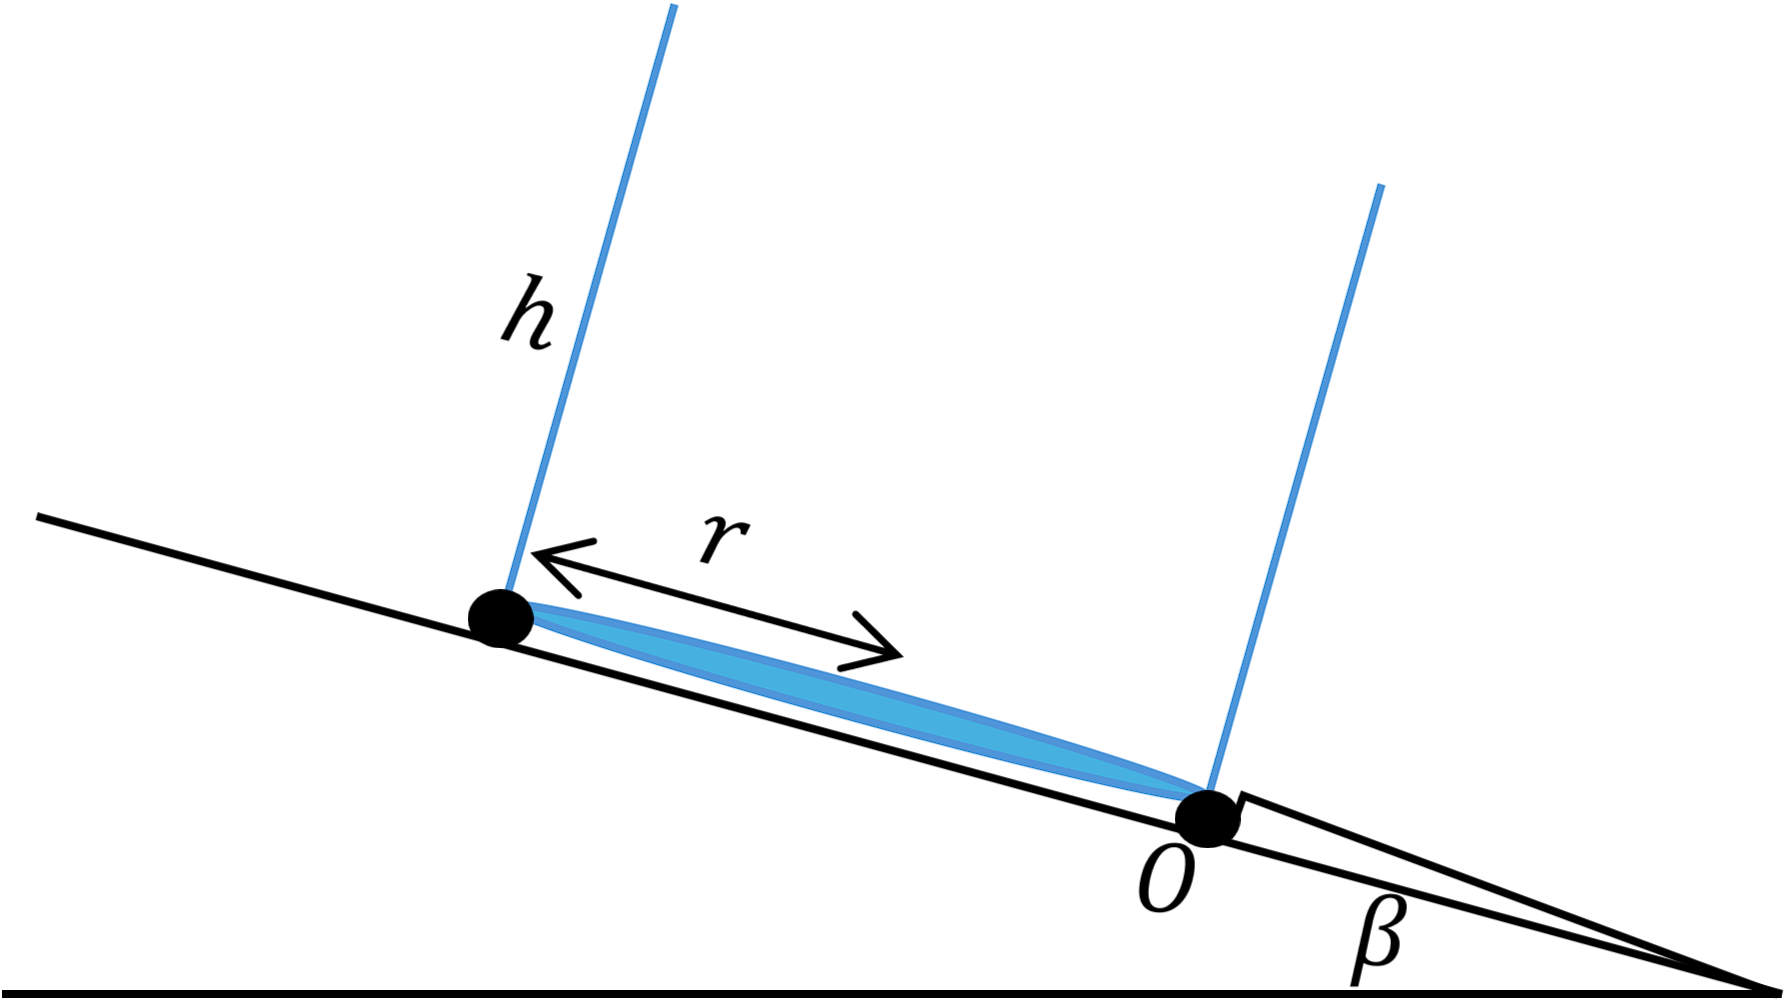
\includegraphics[width=1\linewidth]{tutorías/2024/img/vaso.png}
    \end{figure}    
\end{minipage}
% Para imágenes vectoriales -> el texto tiene que estar en LaTeX
% \begin{figure}[htbp]
%   \centering
%   \svgpath{../Imagenes/ejercicios}  -> .. irse pa'trás 
%   \includesvg{ej5.svg}
% \end{figure}

\end{enumerate}
\end{document}
